\chapter{球員}
\section{繪圖}

\section{組裝}
\begin{figure}[h]
  \begin{center}
    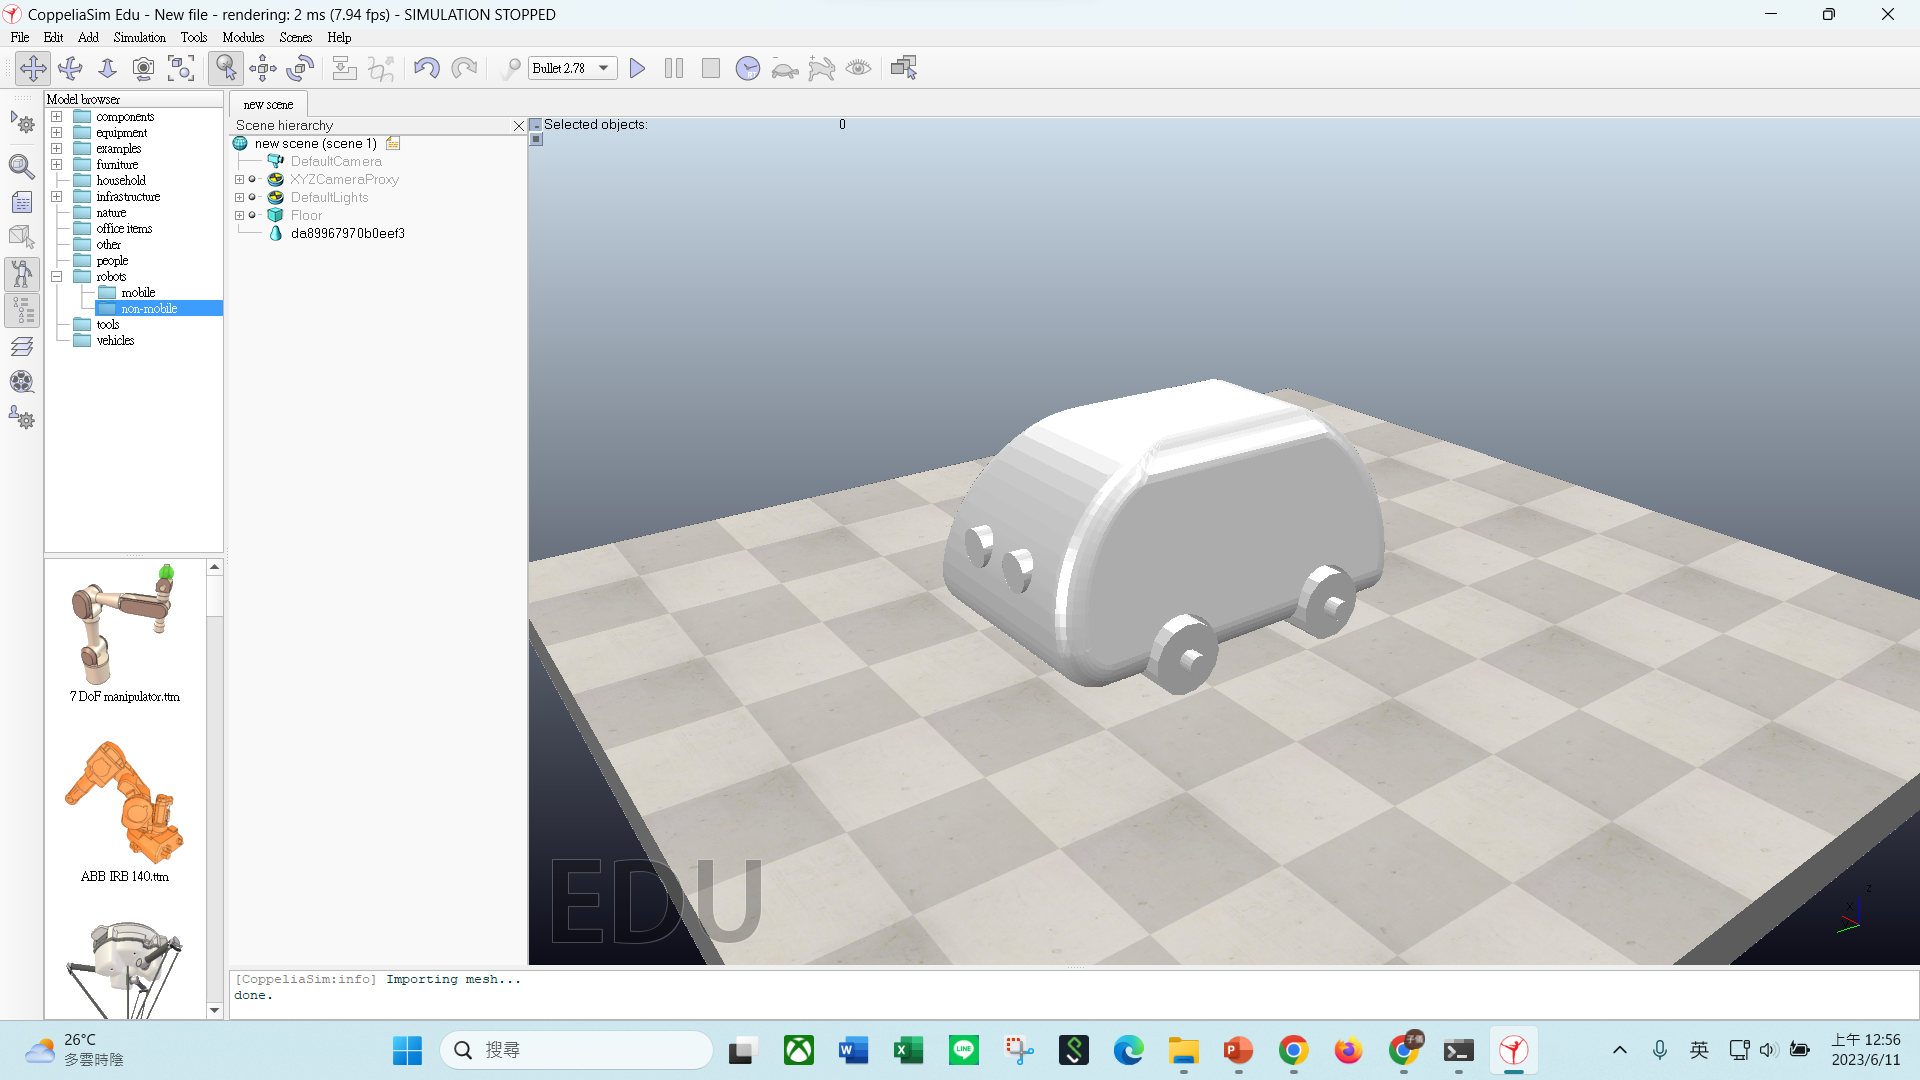
\includegraphics[width=0.5\textwidth]{球員組裝_1.png}
  \end{center}
  \caption{導入球員STL檔}
  \label{fig:photo}
\end{figure}
\begin{figure}[h]
  \begin{center}
    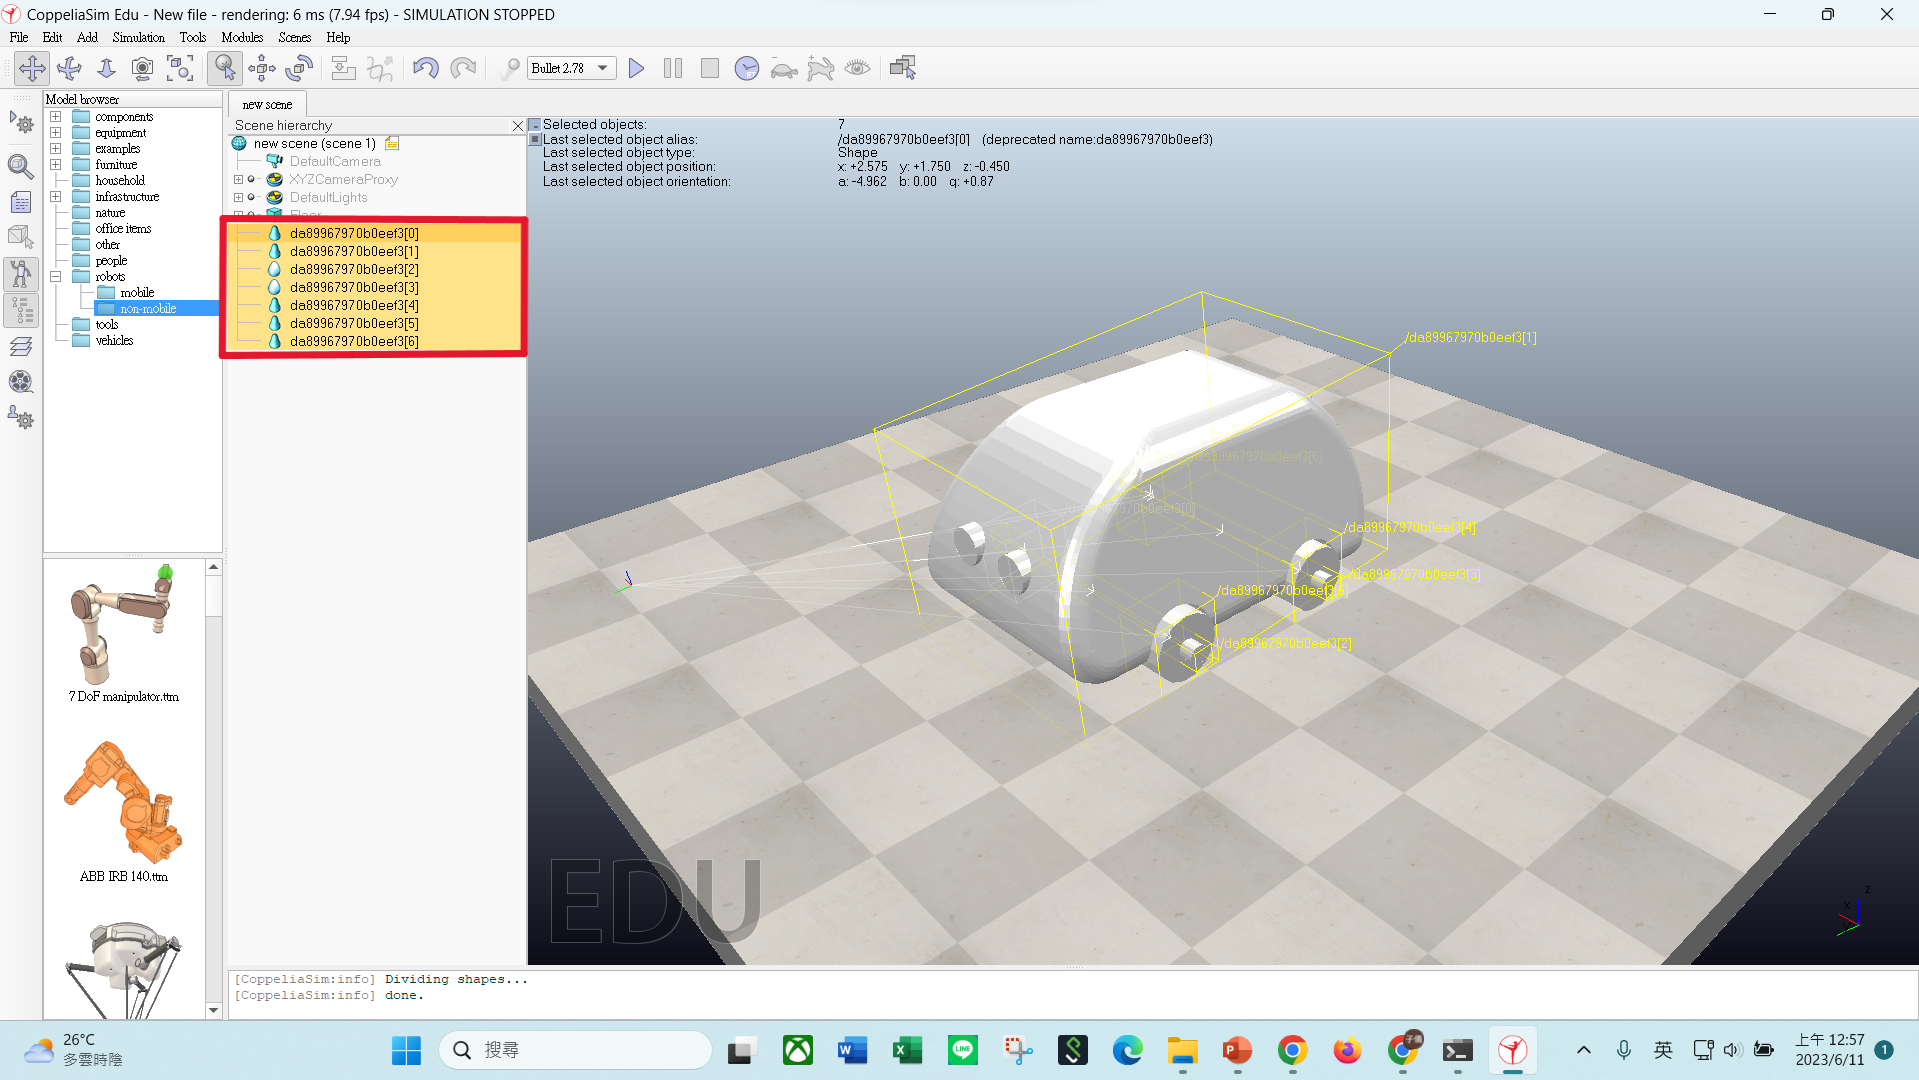
\includegraphics[width=0.5\textwidth]{球員組裝_2.png}
  \end{center}
  \caption{爆炸分解}
  \label{fig:photo}
\end{figure}
\begin{figure}[h]
  \begin{center}
    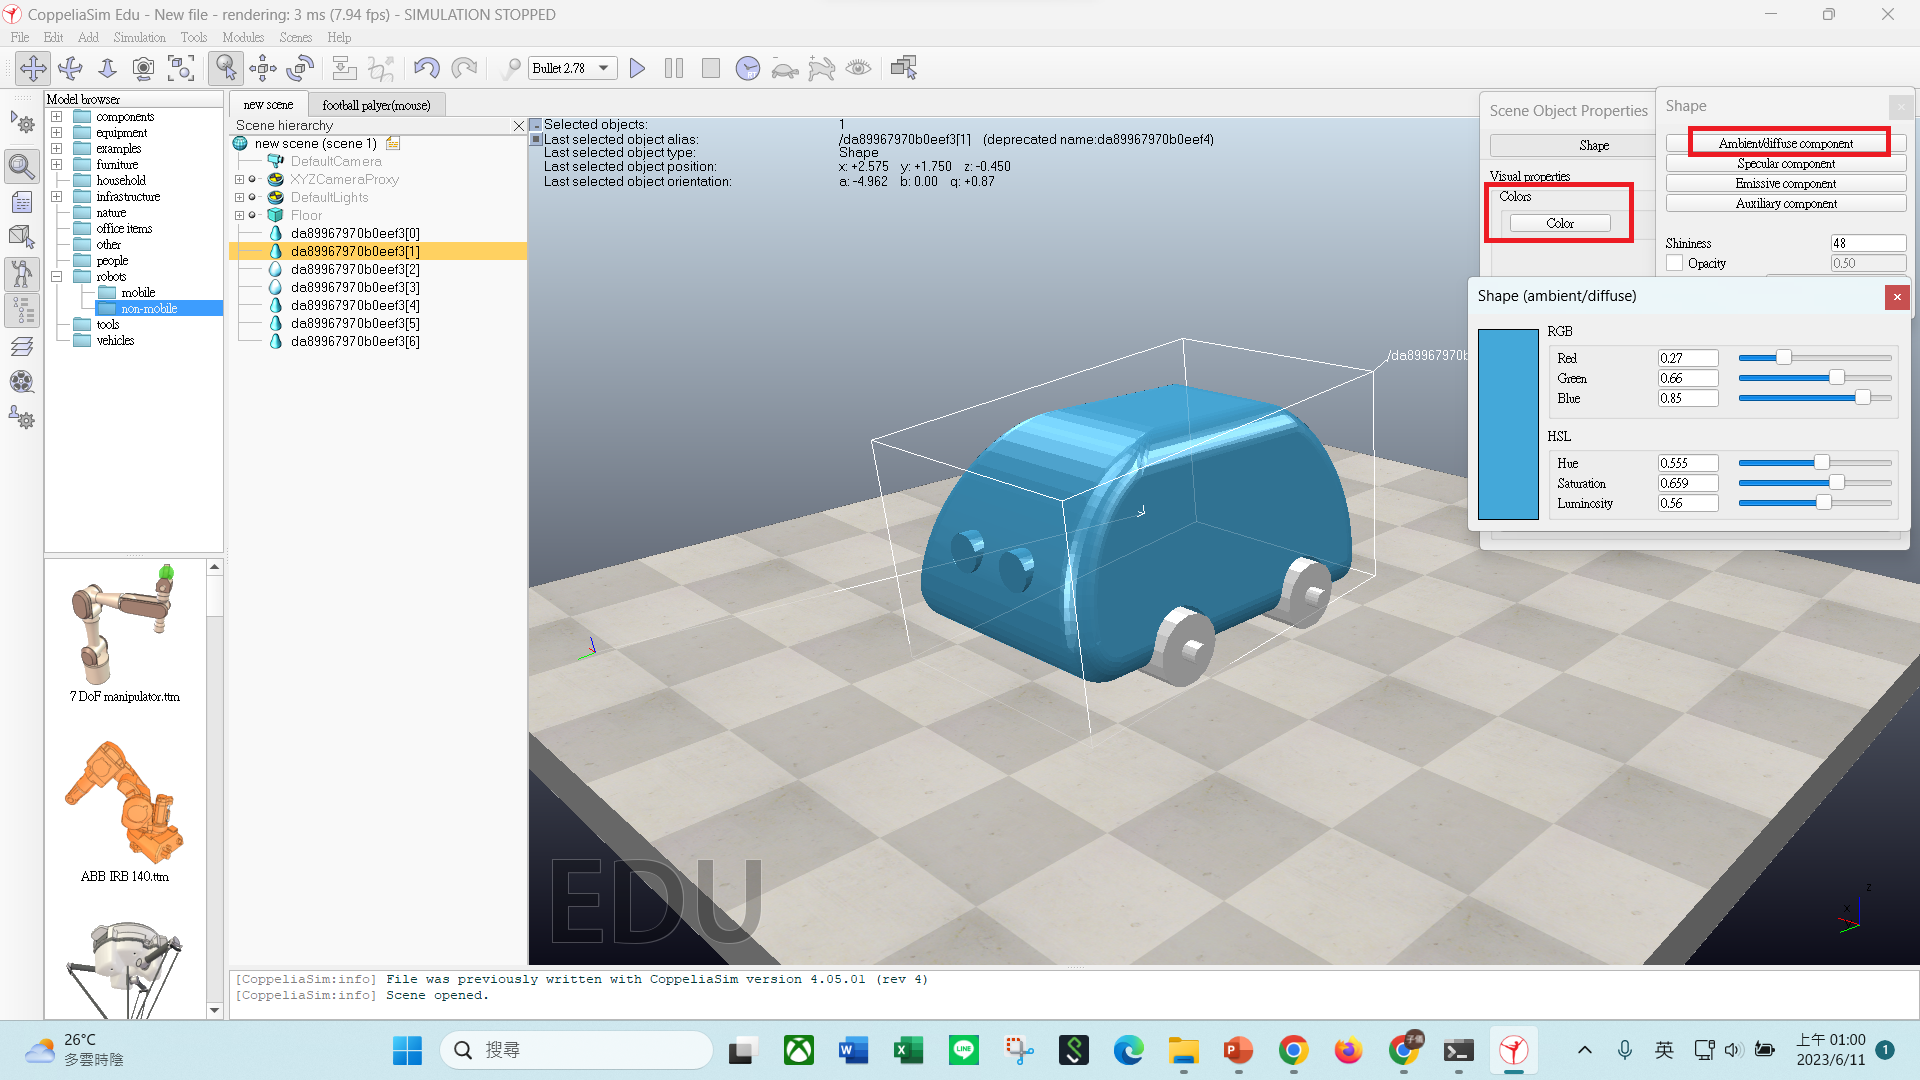
\includegraphics[width=0.5\textwidth]{球員組裝_3.png}
  \end{center}
  \caption{更改顏色}
  \label{fig:photo}
\end{figure}
\begin{figure}[h]
  \begin{center}
    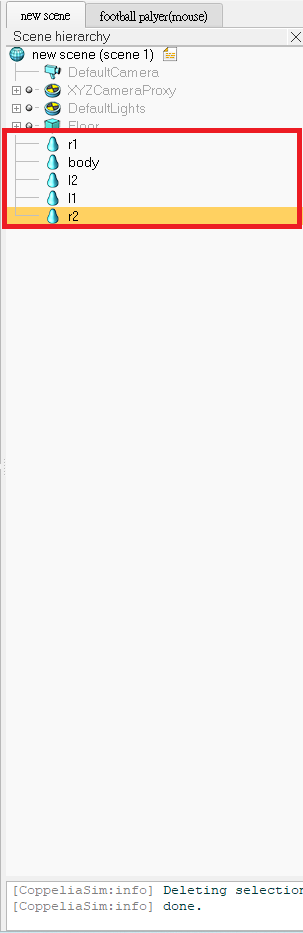
\includegraphics[width=0.5\textwidth]{球員組裝_4.png}
  \end{center}
  \caption{更改物件名稱}
  \label{fig:photo}
\end{figure}
\begin{figure}[h]
  \begin{center}
    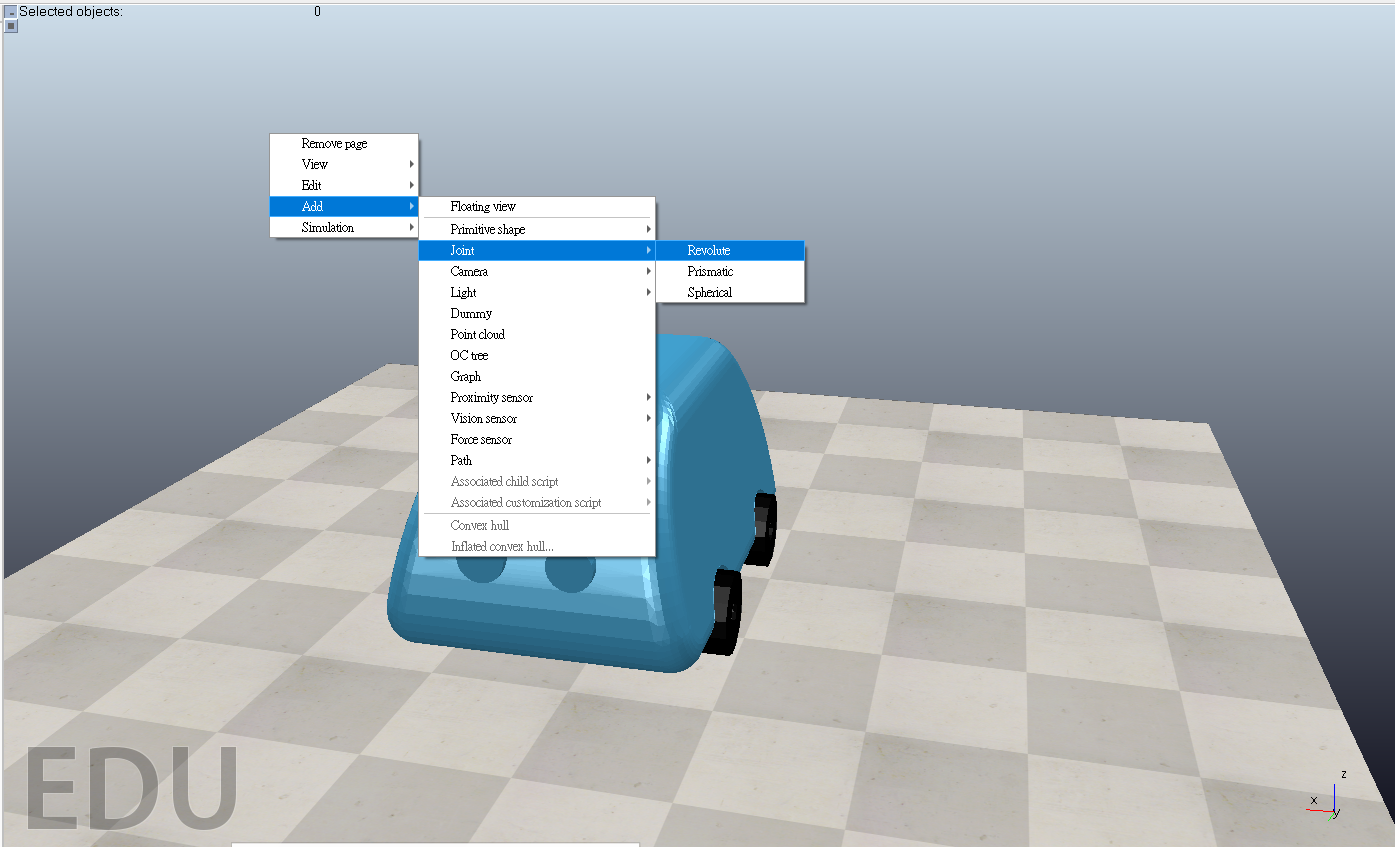
\includegraphics[width=0.5\textwidth]{球員組裝_5.png}
  \end{center}
  \caption{新增Joint}
  \label{fig:photo}
\end{figure}
\begin{figure}[h]
  \begin{center}
    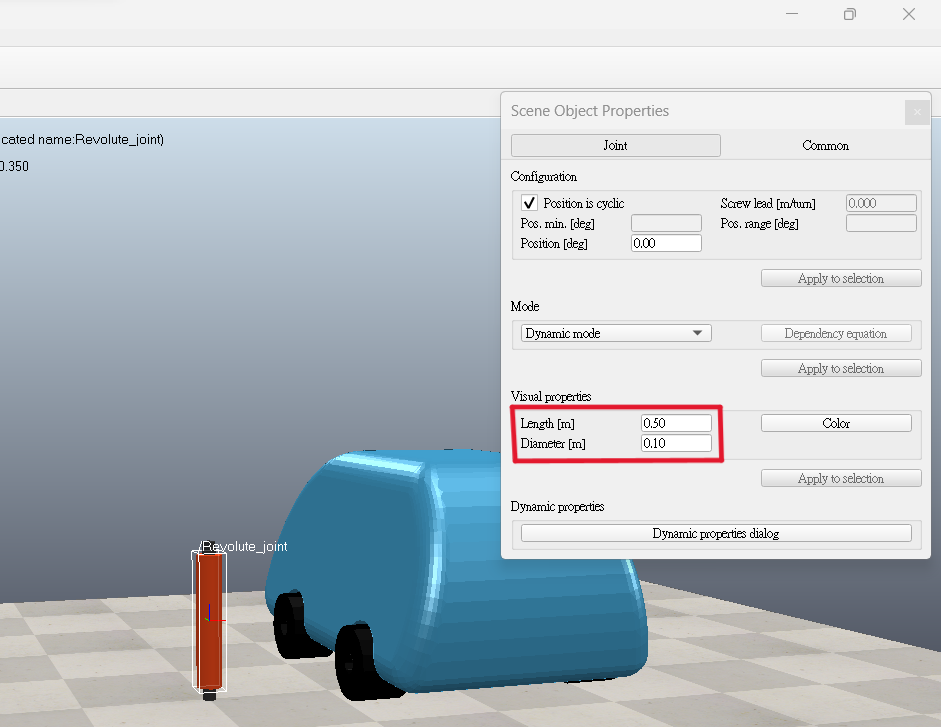
\includegraphics[width=0.5\textwidth]{球員組裝_6.png}
  \end{center}
  \caption{調整Joint大小}
  \label{fig:photo}
\end{figure}
\begin{figure}[h]
  \begin{center}
    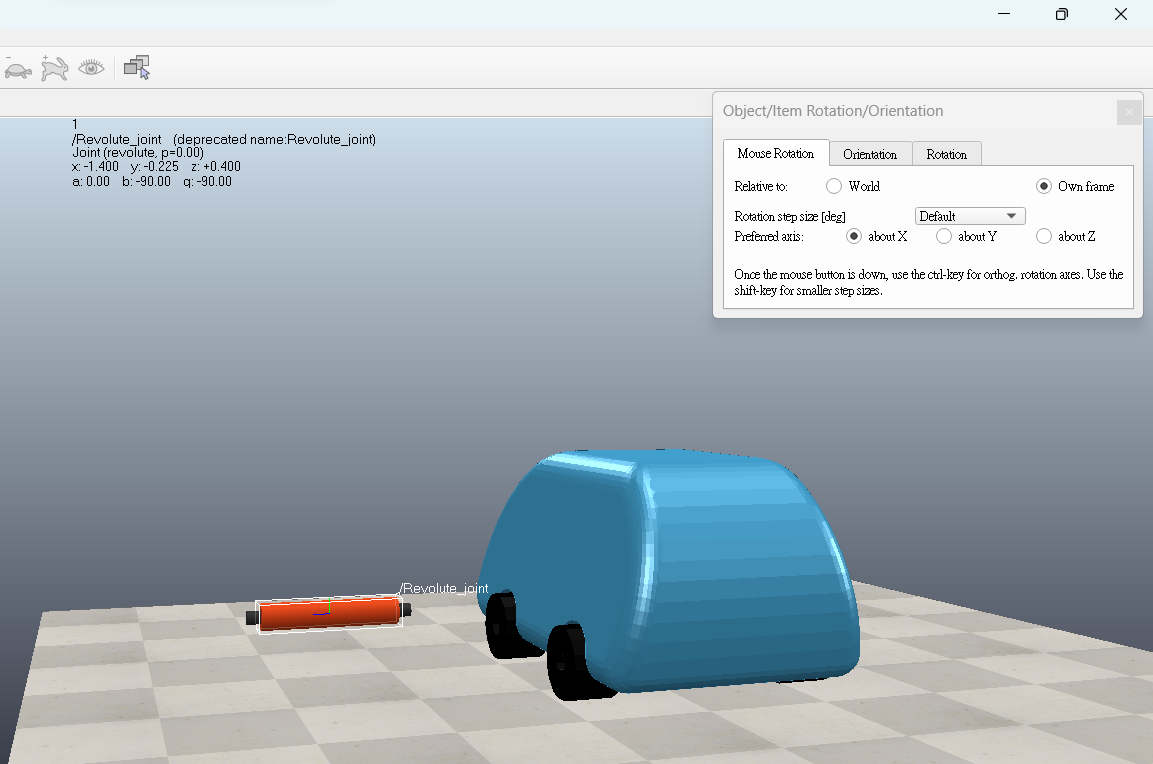
\includegraphics[width=0.5\textwidth]{球員組裝_7.png}
  \end{center}
  \caption{繞X軸旋轉,使Joint與物件平行}
  \label{fig:photo}
\end{figure}
\begin{figure}[h]
  \begin{center}
    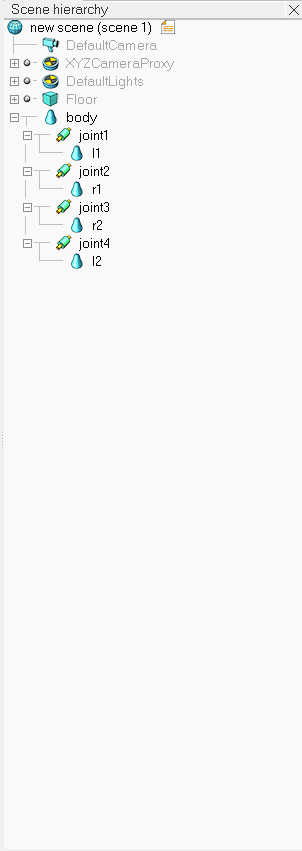
\includegraphics[width=0.5\textwidth]{球員組裝_8.png}
  \end{center}
  \caption{物件相互依附}
  \label{fig:photo}
\end{figure}
\begin{figure}[h]
  \begin{center}
    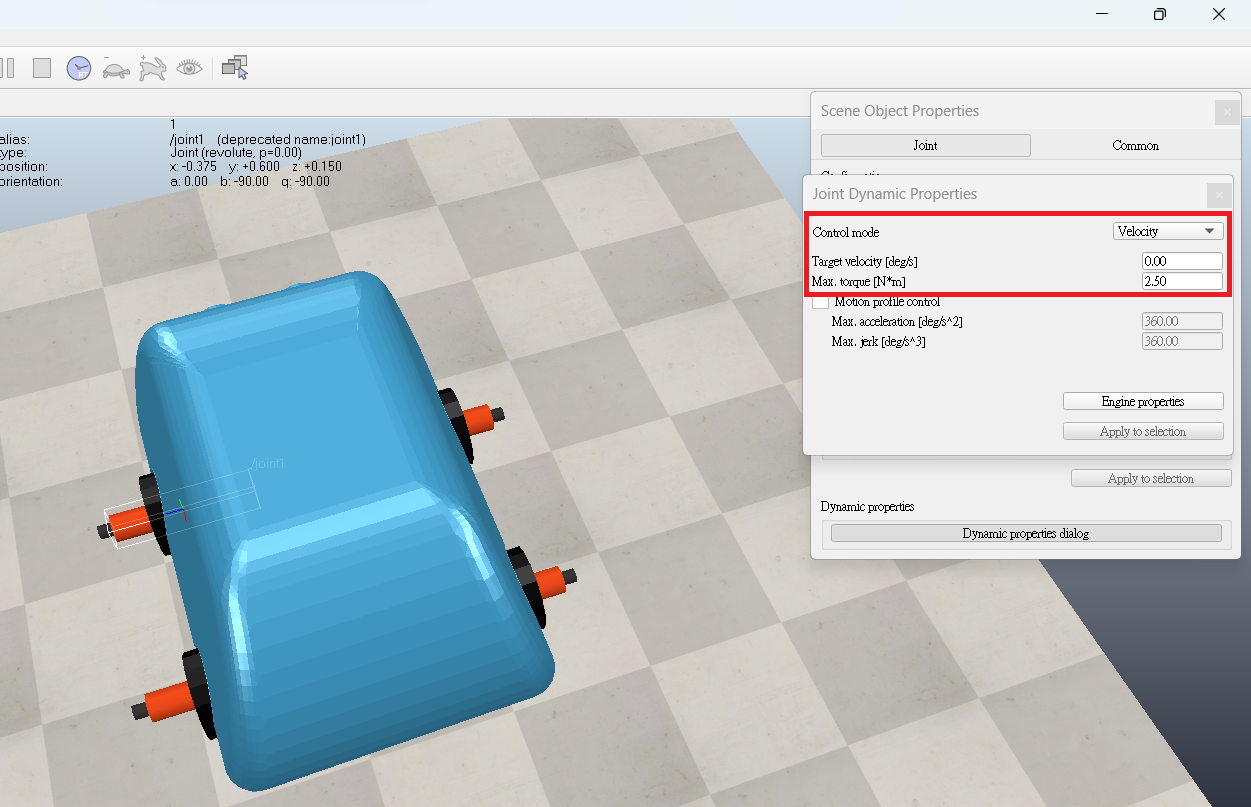
\includegraphics[width=0.5\textwidth]{球員組裝_9.png}
  \end{center}
  \caption{調整物件傳動參數}
  \label{fig:photo}
\end{figure}
\begin{figure}[h]
  \begin{center}
    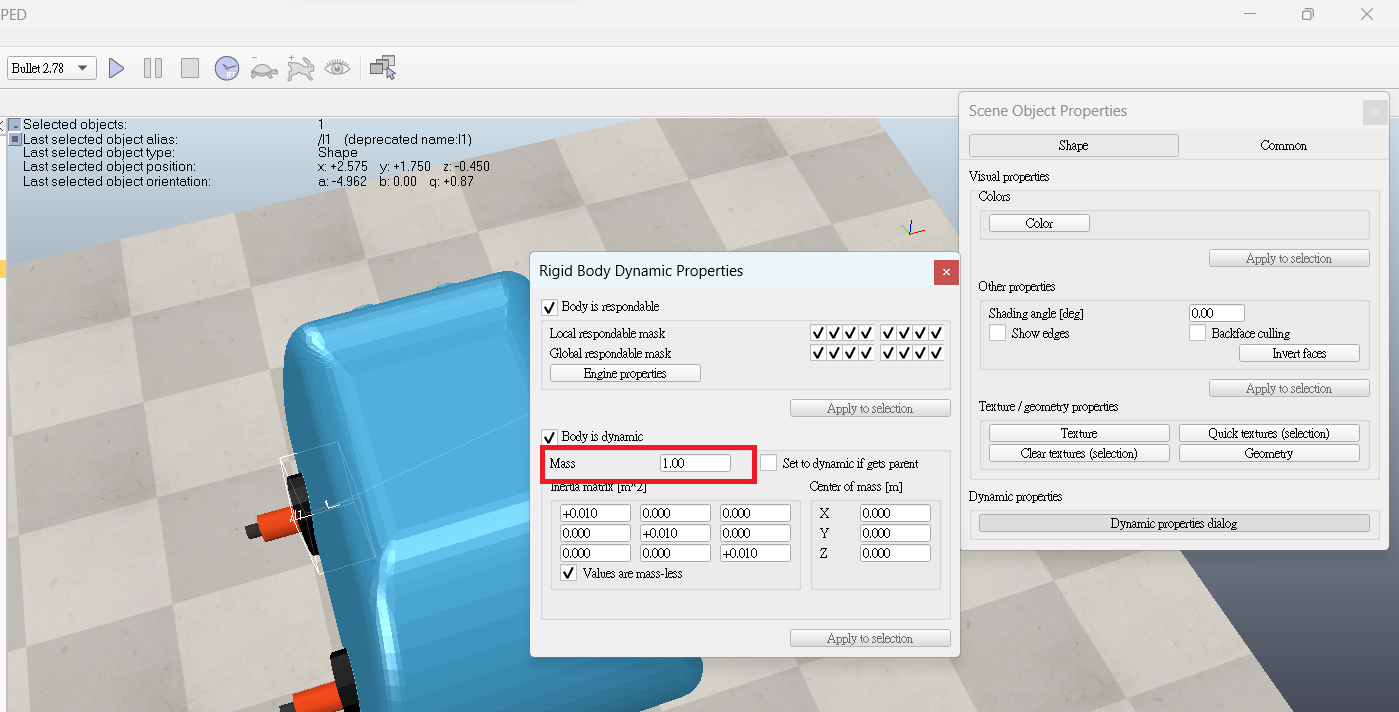
\includegraphics[width=0.5\textwidth]{球員組裝_10.png}
  \end{center}
  \caption{調整物件質量參數}
  \label{fig:photo}
\end{figure}

\section{背號}

\section{程式碼}
